\chapter{Digital Electronics}
\section{Multiplexer(MUX)}
Multiplex means many into one. A multiplexer is a circuit with many inputs but only one output. By applying control signals, we can steer any input to the output. Thus it is also called a data selector and control inputs are termed select inputs. A MUX is represented by many input and single output line.The internal structure of MUX is a rotatory switch.
\\ It is used for parellel to series conversion. It's also called as universal combinational circuit.

\begin{figure}[H]
	\centering
	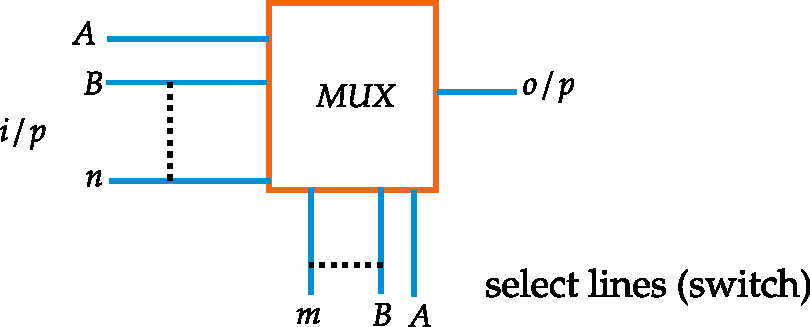
\includegraphics[height=3cm,width=7cm]{EDE-40}
	\caption{}
	\label{}
\end{figure}
If the number of input lines in a MUX is $N$, then,
\begin{align*}
N&=2^n\\
\text{Where, } n&=\text{number of select lines.}
\end{align*}
\subsection{$2 \times 1$ MUX}
Here, the number of input lines,N
\begin{align*}
N&=2^{n}=2\\
\text{Then,number of select lines } n&=1
\end{align*}
\begin{example}
 For a two level AND-OR circuit can be equally represented by
	\begin{tasks}(2)
		\task[\textbf{a.}]AND-AND
		\task[\textbf{b.}]OR-AND
		\task[\textbf{c.}]NOR-NOR
		\task[\textbf{d.}] NAND-NAND
	\end{tasks}

		\begin{figure}[H]
			\centering
			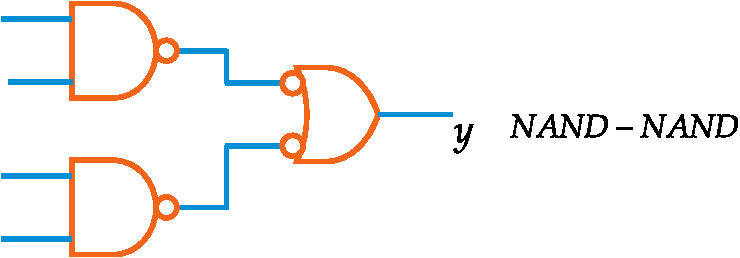
\includegraphics[height=2.4cm,width=7cm]{EDE-42}
		\end{figure}
	
\end{example}
\subsection{4$\times$ 1 MUX}
\begin{figure}[H]
	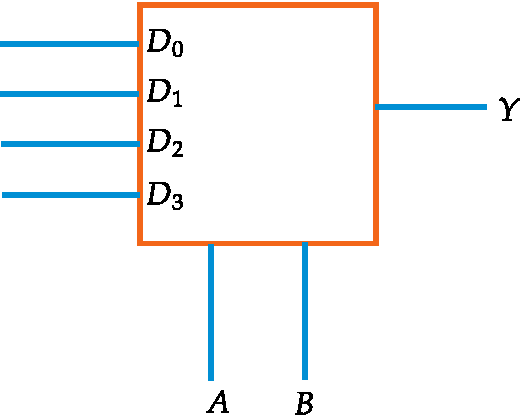
\includegraphics[height=3.5cm,width=4.5cm]{DE-01}
\end{figure}
\text{Output }\quad y=$\bar{A}\bar{B}D_0+\bar{A}BD_1+A\bar{B}D_2+ABD_3$
\subsection{8$\times 1$ MUX}
\begin{align*}
	2^n&=8\\
	\Rightarrow &\text{ number of select lines, }n=3\\
	y&=\bar{A}\bar{B} \bar{C}D_0+\bar{A}\bar{B} CD_1+
	\bar{A}B\bar{C}D_2+\bar{A}BCD_3+
	A \bar{B}\bar{C}D_4+A\bar{B}CD_5+
	AB\bar{C}D_5+ABCD_7
\end{align*}
\section
{Minimization of logical expression of using MUX:}
1.\quad  Minimize
\begin{figure}[H]
	\centering
	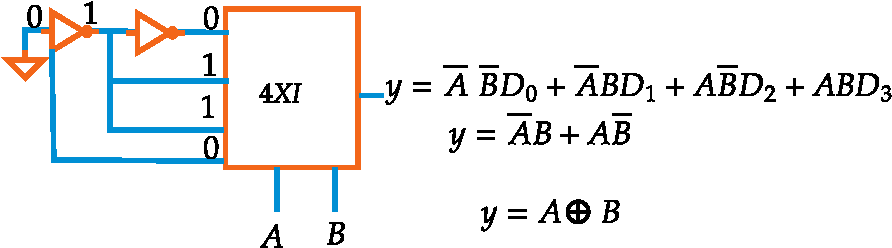
\includegraphics[height=2.7cm,width=9cm]{EDE-43}
\end{figure}
2.\quad  Minimize
\begin{figure}[H]
	\centering
	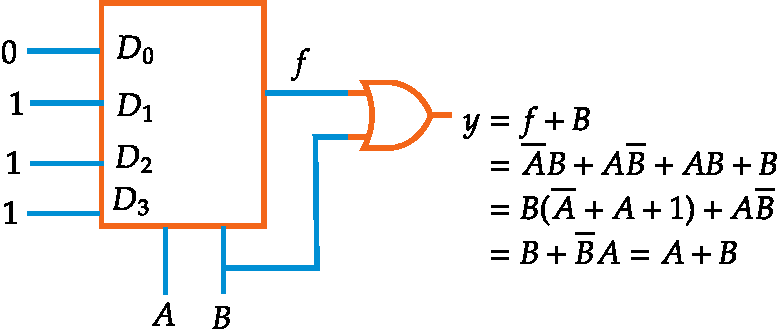
\includegraphics[height=3.2cm,width=8.5cm]{EDE-44}
\end{figure}
\subsection{Implementation of higher order MUX by using $2\times 1$MUX:}
\begin{enumerate}
	\item $4\times1$ MUX by $2\times 1$ MUX
	\begin{figure}[H]
		\centering
		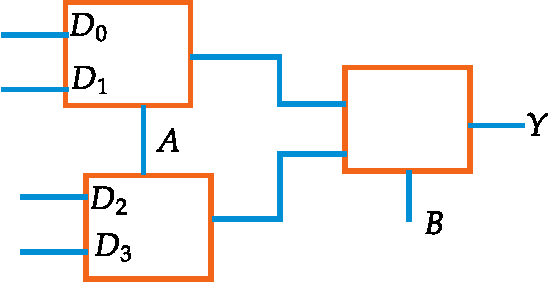
\includegraphics[height=3cm,width=5cm]{EDE-45}
	\end{figure}
	\begin{align*}
	\text{Alternate method to find the number of MUX}\\
	\begin{tabular}{p{0.5cm}|p{0.5cm}}
	2&4\\\hline
	2&2\\\hline
	&1
	\end{tabular}\\
	2+ 1=3\\
	\text{ three, } 2 \times 1\text{ MUX } \text{is required}
	\end{align*}
 $16\times 1$ MUX by $2\times 1$ MUX
	\begin{align*}
	\begin{array}{c|c}
	2 & 16 \\
	\hline 2 & 8\\
\hline	2 & 4 \\
	\hline 2 & 2 \\
	\hline & 1
	\end{array}=8+4+2+1\Rightarrow 15, (\text{Fifteen,}\quad 2 \times 1\text{ MUX
		Required.})
	\end{align*}
	similarly,
	\item $256 \times 1$ MUX by $16 \times 1$ MUX
	\begin{align*}
	\begin{tabular}{c|c}
	16 & 256 \\
	\hline 16 & 16\\
	\hline  &1
	\end{tabular}\quad 16+1=17 (\text{Seventeen, }16 \times 1 \text{MUX is required}) .
	\end{align*}
\end{enumerate}
\subsubsection{Implementation of Logic gates by using $2 \times 1$ MUX and $u \times 1$ MUX:}
1.\quad NOT gate:
\begin{figure}[H]
	\centering
	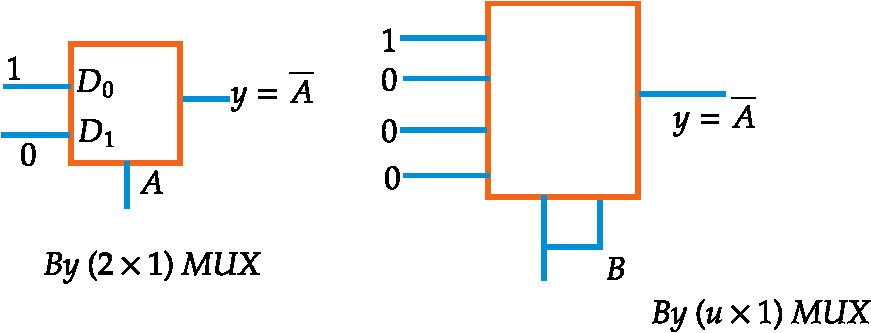
\includegraphics[height=2.8cm,width=4.5cm]{EDE-46}
\end{figure}
\renewcommand*{\arraystretch}{1.5}
$\begin{array}{|c|c|c|}
\hline\text { Logic gate } & \text { 2$\times$1 MUX } & \text { 4$\times$1 MUX } \\
\hline \text { NOT } & 1 & 1 \\
\hline \text { AND } & 1 & 1 \\
\hline \text { OR } & 1 & 1 \\
\hline \text { NAND } & 2 & 1\\
\hline \text { NOR } & 2 & 1\\
\hline \text { EX-OR } & 2 & 1\\
\hline \text { EX-NOR } & 2 & 1\\	\hline
\end{array}$\\\\\\
2. \quad For the implementation of AND gate and XOR gate the number of 2X1 MUX required.
\begin{tasks}(4)
	\task[\textbf{a.}] 1,1
	\task[\textbf{b.}]1,2
	\task[\textbf{c.}]2,1
	\task[\textbf{d.}] 2,2
\end{tasks}
\begin{answer}
	\begin{align*}
	\text { I MUX for AND, 2MUX for XOR }
	\end{align*}
	So the correct answer is \textbf{Option (b)}
\end{answer}
\subsubsection{Demultiplexer:}
A de MUX performs the reverse operation of MUX.
\begin{figure}[H]
	\centering
	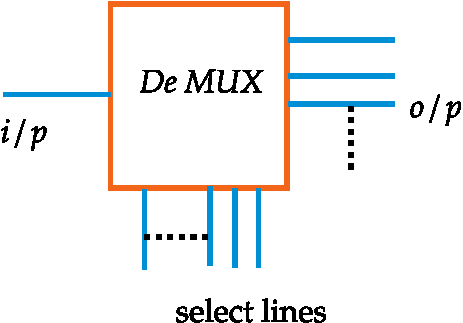
\includegraphics[height=3.3cm,width=4.7cm]{EDE-47}
\end{figure}
\begin{itemize}
	\item Number of outputs $=2^{n}$ where $n \rightarrow$ select lines
	\item  De MUX is also called as data detector.
	\item By setting the input to true (1), the demux behaves as decoder.
\end{itemize}
\subsubsection{$1 \times 4$ DEMUX}
\begin{figure}[H]
	\centering
	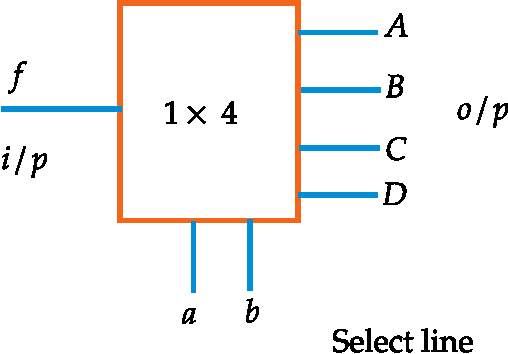
\includegraphics[height=3.5cm,width=5.1cm]{EDE-48}
\end{figure}
\section{Flip-Flop}
\subsubsection{Sequential Circuit}
Digital output are required to be generated in accordance with sequence in which input signals are received, which is not possible with the combinational circuit generated should depend on present and past history of input. Such circuit is called as sequential circuit.\\\\
	\subsubsection{SR-Latch:}
	\begin{figure}[H]
		\centering
		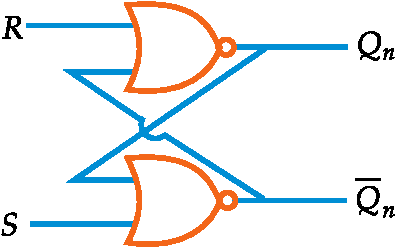
\includegraphics[height=2.8cm,width=4.5cm]{EDE-01}
	\end{figure}
\subsubsection{Truth Table:}
\begin{tabular}{|c|c|c|c|}
	\hline$C L K$ & $R$ & $S$ & $Q_{n+1}$ \\
	\hline 1 & 0 & 0 & $Q_{n}$ \\
	\hline 1 & 0 & 1 & 1 \\
	\hline 1 & 1 & 0 & 0 \\
	\hline 1 & 1 & 1 & Invalid \\
	\hline 0 & $X$ & $X$ & $Q_{n}$ \\
	\hline
\end{tabular}
$\mathrm{X}$ : Input either 0 or 1
\subsubsection{ S-R Flip Flop with NAND Gate: }
\begin{figure}[H]
	\centering
	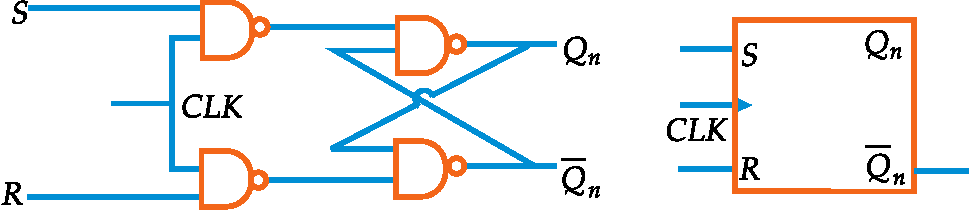
\includegraphics[height=2.1cm,width=11cm]{EDE-02}
\end{figure}
\subsubsection{D-Flip Flop (Delay): }
When $\mathrm{S}=\mathrm{D}, \bar{R}=D$, Now SR becomes $\mathrm{D}$ type Flip Flop.
\begin{figure}[H]
	\centering
	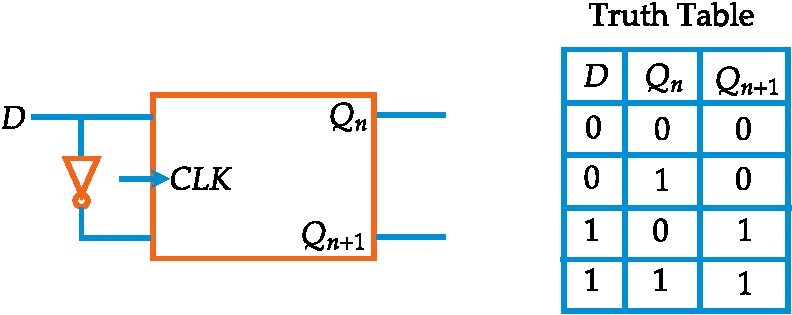
\includegraphics[height=3.2cm,width=7.7cm]{EDE-03}
\end{figure}
\subsubsection{ J-K Flip Flop: }
$S=J\left(\bar{Q}_{n}\right) ; R=K\left(Q_{n}\right)$
\begin{figure}[H]
	\centering
	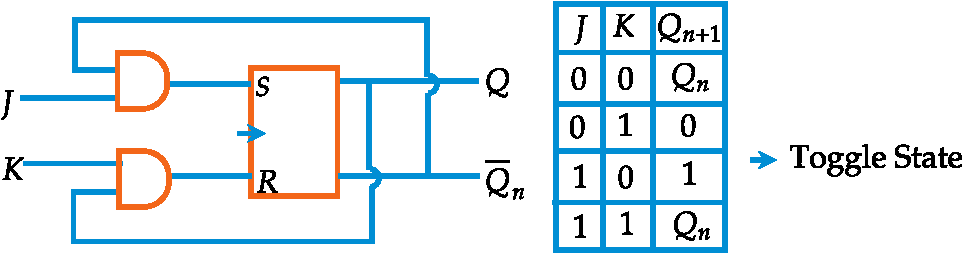
\includegraphics[height=2.4cm,width=9.5cm]{EDE-04}
\end{figure}
\begin{note}
Problem in JK flip flop is race around condition.
\end{note}
\subsubsection{T-type (Toggle) Flip Flop:} $\mathrm{J}=\mathrm{K}=\mathrm{T}$ then $\mathrm{T}=$ Flip Flop.
 \begin{figure}[H]
 	\centering
 	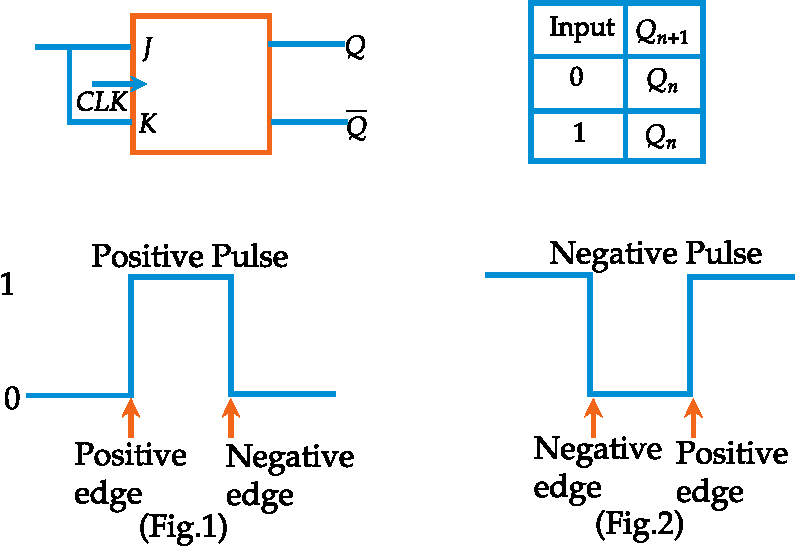
\includegraphics[height=5.4cm,width=7.5cm]{EDE-05}
 \end{figure}
 A clock pulse may be either positive or negative. A positive clock source remains at 0 during the interval between pulses and goes 0 to 1 during the occurrence of a pulse. The pulse goes through two signal transitions; from 0 to 1 and return from 1 to 0, positive transition is defined as the positive edge and the negative transition as the negative edge.\\
\subsubsection{Time Diagram Representation:}
 \begin{figure}[H]
 	\centering
 	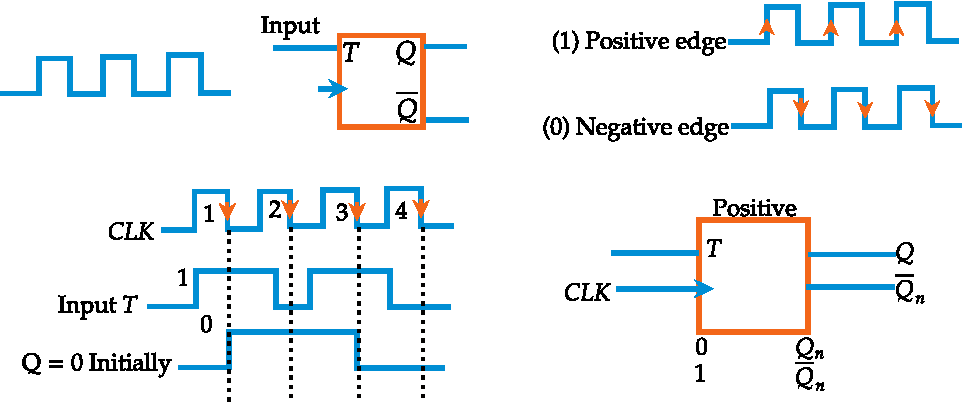
\includegraphics[height=4.8cm,width=10.5cm]{EDE-06}
 \end{figure}
\subsubsection{If we take positive edge:}
 \begin{figure}[H]
 	\centering
 	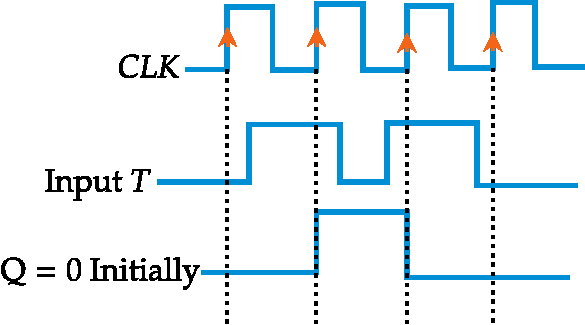
\includegraphics[height=3cm,width=5.4cm]{EDE-07}
 \end{figure}
 	\textbf{Counters}
 	\begin{enumerate}
 		\item Asynchronous or ripple or serial 
 		\item Synchronous or parallel or fast
 		\item (i) Ring counter (ii) Twisted tail or thomson or mobious (Type of shift registers)
 	\end{enumerate}
 \begin{enumerate}
 	\item \textbf{Asychronous Counter:} No, common clock-clock is output of previous flip-flop.
 	\item In synchronous counter common clock is used.
 \end{enumerate}
\begin{enumerate}
\item  	What is meaning of MOD-12 counter $\Rightarrow$ number of states are 12 .\\
1. $0-11 \rightarrow 12$ states\qquad
2. $2-13 \rightarrow 12$ states\\
3. $3-14 \rightarrow 12$ states\qquad
4. $1-12 \rightarrow 12$ states\\
 	MOD 12 means divide by 12 .
 	\begin{figure}[H]
 		\centering
 		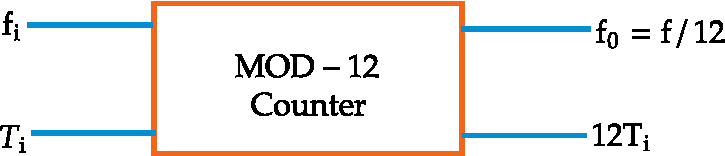
\includegraphics[height=1.3cm,width=6cm]{EDE-13}
 	\end{figure}
 \subsubsection{ Asynchronous Counter: }
 		\begin{figure}[H]
 		\centering
 		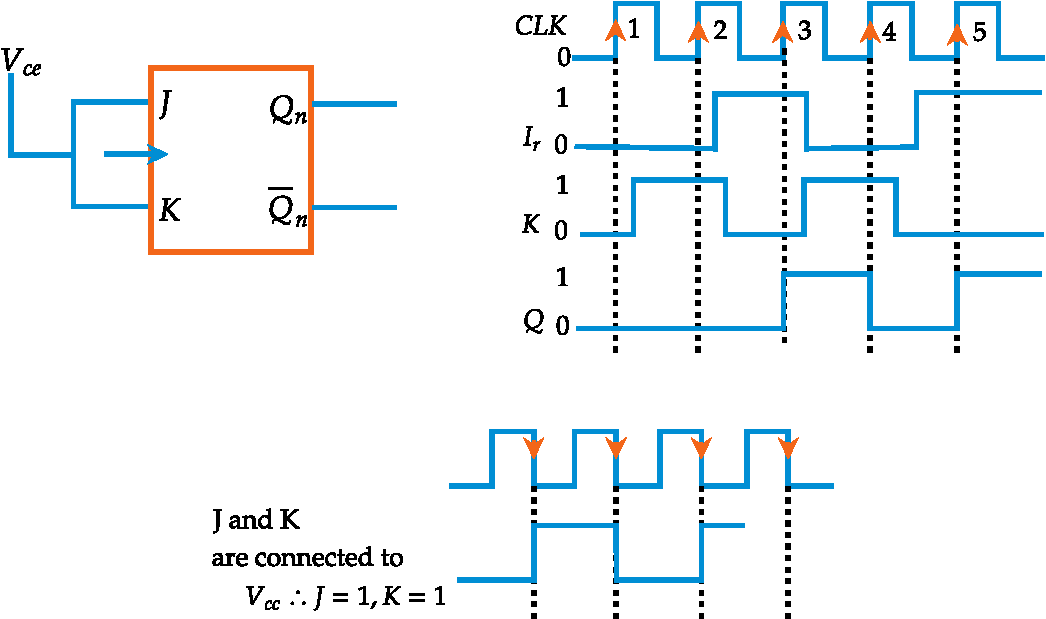
\includegraphics[height=6cm,width=10cm]{EDE-14}
 	\end{figure}
 \begin{note}
 		1. Total number of flip-flop required for Mod-N counter $\mathrm{N}=2^{n}$.\\
 	2. 3 bit means MOD-8 counter $\Rightarrow$ MOD $8=2^{3}$ means 3 Flip-Flop required.\\
 	3. 4 bit $\rightarrow 16 \mathrm{MOD} \rightarrow 2^{4} \rightarrow 4$ Flip Flop required
 \end{note}
 \subsubsection{ MOD-8 Asychronous Counter: }
 	\begin{figure}[H]
 		\centering
 		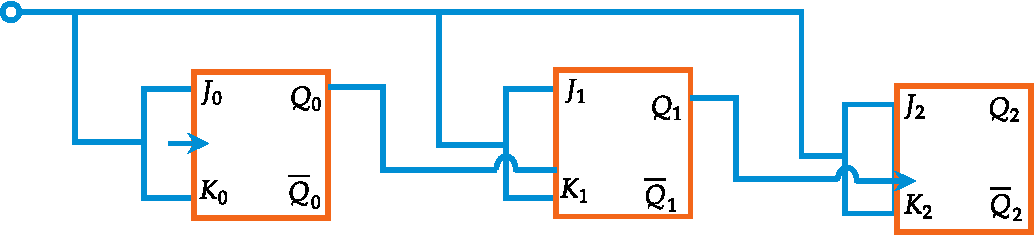
\includegraphics[height=2.3cm,width=9cm]{EDE-15}
 	\end{figure}
 \begin{figure}[H]
 	\centering
 	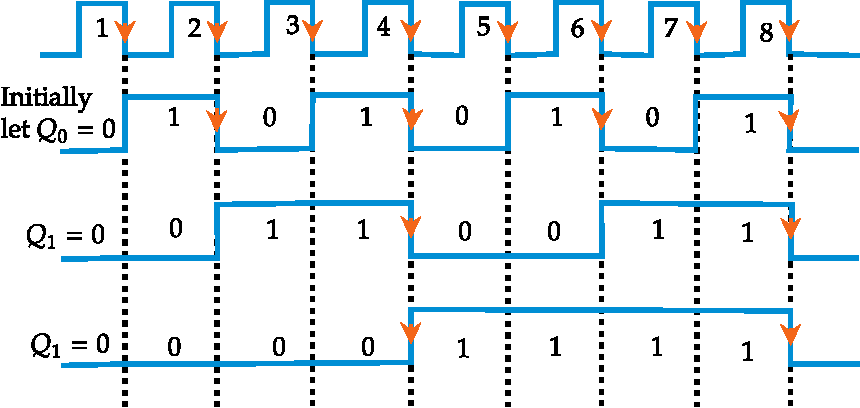
\includegraphics[height=5cm,width=10cm]{EDE-16}
 \end{figure}
\begin{align*}
	&\text { Truth Tuble }\\
	&\begin{array}{|c|c|c|c|}
		\hline C L K & Q_{2} & Q_{1} & Q_{0} \\
		\hline 1 & 0 & 0 & 0 \\
		\hline 2 & 0 & 0 & 1 \\
		\hline 3 & 0 & 1 & 0 \\
		\hline 4 & 0 & 1 & 1 \\
		\hline 5 & 1 & 0 & 0 \\
		\hline 6 & 1 & 0 & 1 \\
		\hline 7 & 1 & 1 & 0 \\
		\hline 8 & 1 & 1 & 1 \\
		\hline
	\end{array}
\end{align*}
 	Edge $\rightarrow$ Positive $\rightarrow$ (i) up counter (ii) Down counter \\
 	Edge $\rightarrow$ Negative $\rightarrow$ (i) up counter (ii) Down counter
 	\begin{figure}[H]
 		\centering
 		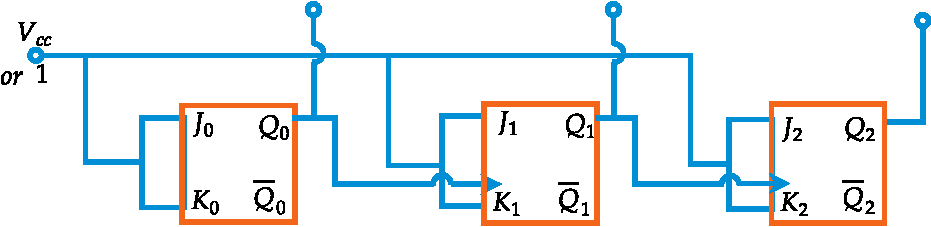
\includegraphics[height=2.5cm,width=9.5cm]{EDE-17}
 	\end{figure}
 	$\mathrm{Q}_{2}, \mathrm{Q}_{1}, \mathrm{Q}_{0}$ are standard output\\
 	\textbf{Case (i):} If the output is of first flip-flop is given as circuit to next flip-flop it will act as up counter.\\
 	\textbf{Case (ii):} If $\bar{Q}$ of 1 st flip flop is given as circuit to next flip-flop it will act as down counter.
 	\begin{figure}[H]
 	\centering
 	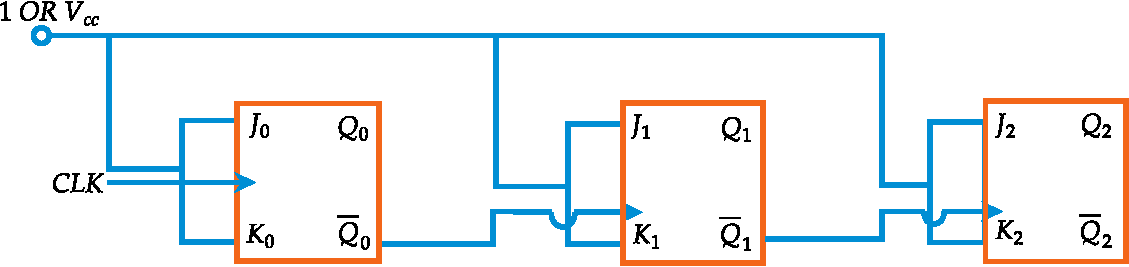
\includegraphics[height=2.6cm,width=9.8cm]{	EDE-18}
 \end{figure}
\subsubsection{Synchronous Counter}
(i) Common clock is there (ii) There are fast \\
Widely used if MOD is in form of 2N then design is simple. If MOD is not in form of 2N then design by use of K-map.\\
	Example: MOD-10 UP counter.
	\begin{figure}[H]
		\centering
		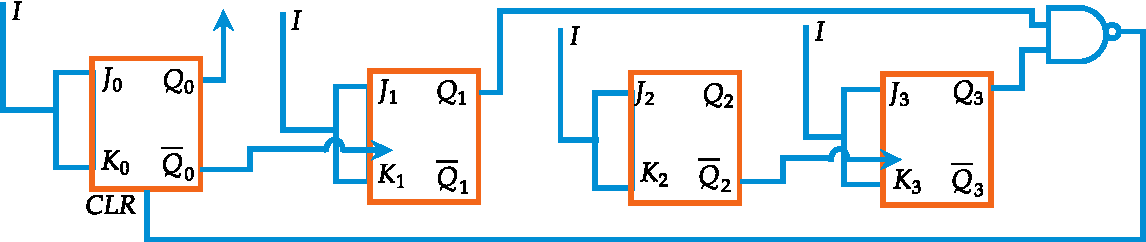
\includegraphics[height=2.5cm,width=12cm]{EDE-21}
	\end{figure}
\begin{figure}[H]
	\centering
	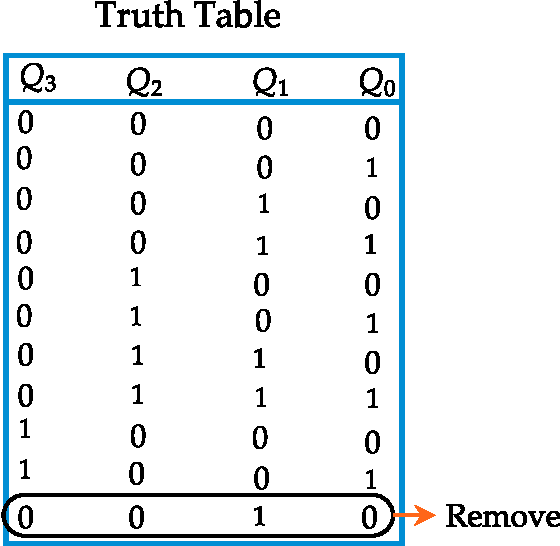
\includegraphics[height=5cm,width=4.5cm]{EDE-22}
\end{figure}
\subsubsection{SHIFT REGISTER}
Register's are group of flip-flop.\\
To store $n$-bits $n$-bits $n$-flip-flop are required in register. \\
Depending upon input and output registers can be classified as\\
(1) SISO [Serial input serial output]\quad
(3) PISO [Parallel in serial output]\\
(2) SIPO [Serial input parallel out]\quad
(4) PIPO [Parallel input parallel output]\\
\subsubsection{ 4-Bit SISO}
\begin{figure}[H]
	\centering
	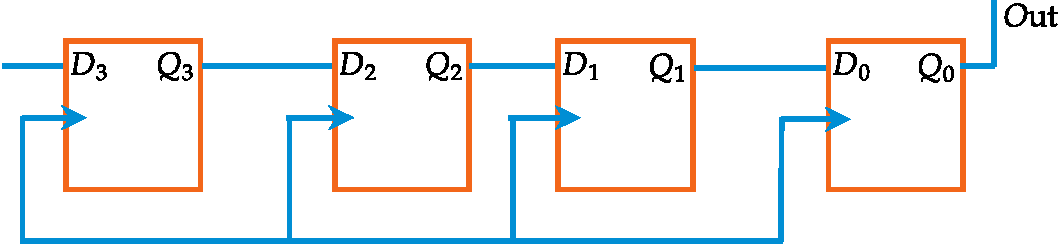
\includegraphics[height=2.4cm,width=10cm]{EDE-27}
\end{figure}
To provide $n$-bit data in $(n-1)$-clk pulse required, \\
To store $n$-bit data $n$-click pulse required.\\
S\subsubsection{IPO(4-Bit)}
\begin{figure}[H]
	\centering
	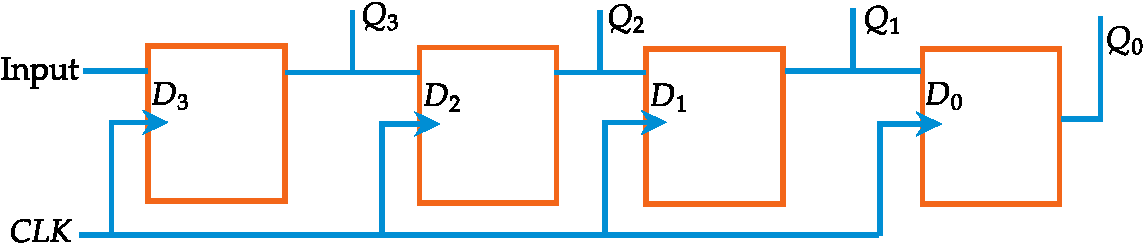
\includegraphics[height=2.2cm,width=10cm]{EDE-28}
\end{figure}
To provide $n$-bit data in $n$-clk pulse required, to provide parallel out no circuit pulse required.\\
\subsubsection{ PISO }
\begin{figure}[H]
	\centering
	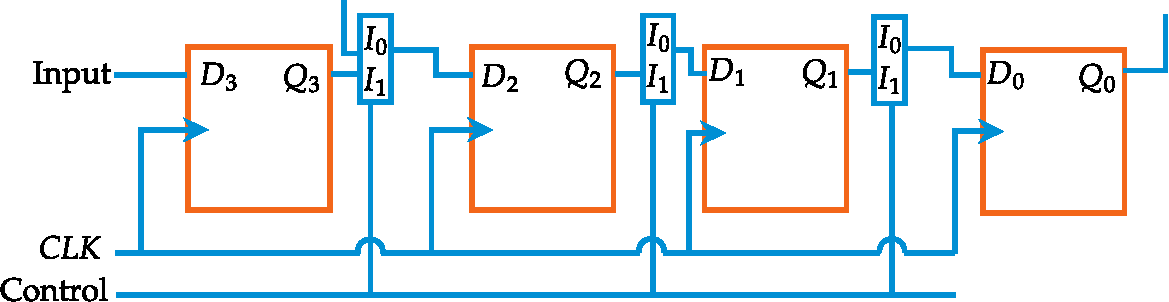
\includegraphics[height=2.6cm,width=10cm]{EDE-29}
\end{figure}
Control $0 \rightarrow$ Parallel input, Control $1 \rightarrow$ Serial output\\
\subsubsection{ PIPO}
\begin{figure}[H]
	\centering
	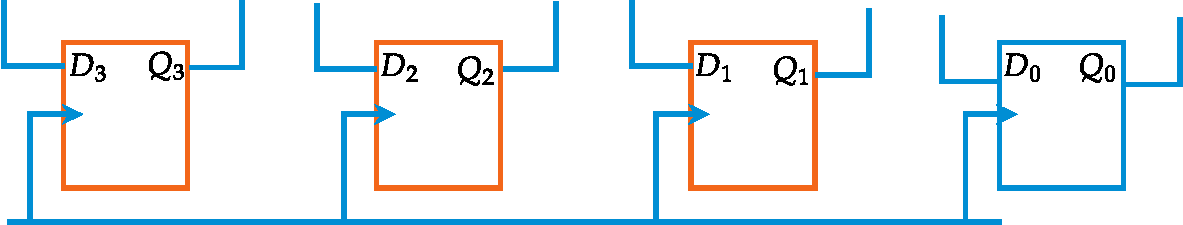
\includegraphics[height=2cm,width=10cm]{EDE-30}
\end{figure}
 Initial contents of 4-bit SIPO, ring shift register, shown in figure is 0110 . After 3 clock pulses are applied, what are contents of shift register.
\begin{figure}[H]
	\centering
	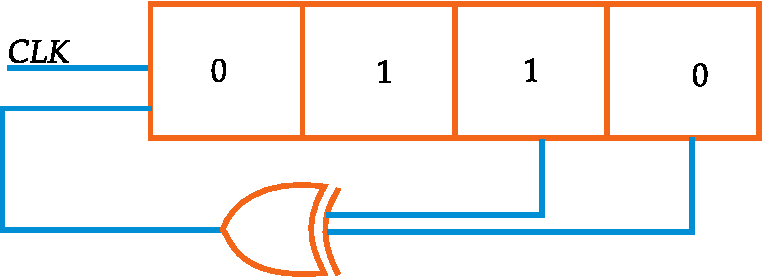
\includegraphics[height=2.4cm,width=6cm]{EDE-31}
\end{figure}
\begin{answer}
	After 1 st clock $\rightarrow 1011,2$ nd clock $\rightarrow 0101$, 3rd clock $\rightarrow 1010$. So content are 1010 .
\end{answer}
\subsubsection{Ring Counter:}
Design MOD-5 ring counter. After each 10 steps is reads again 0000.
\begin{figure}[H]
	\centering
	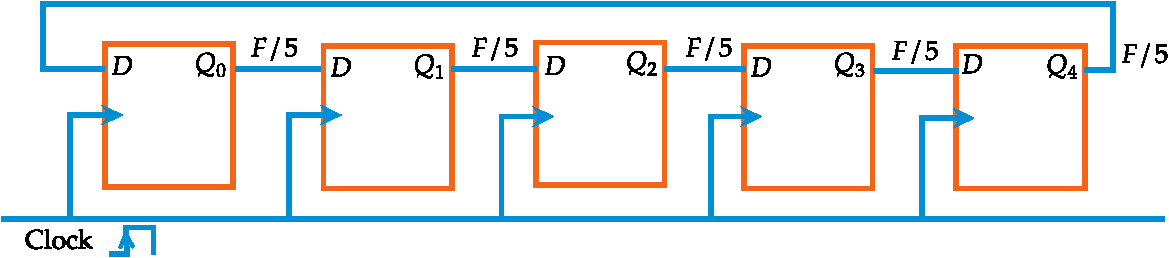
\includegraphics[height=2.6cm,width=11cm]{EDE-34}
\end{figure}
Ring counter is shift register with feedback applied last flip-flop output $Q$ to input of first flip flop.\\
Ring counter is one bit is logic one and it will rotate with clock.\\
In $n$-bit ring counter number of use state is $n$.\\
Number of unused states in $n$-bit ring counter is $2^{n}-n$.
\begin{figure}[H]
	\centering
	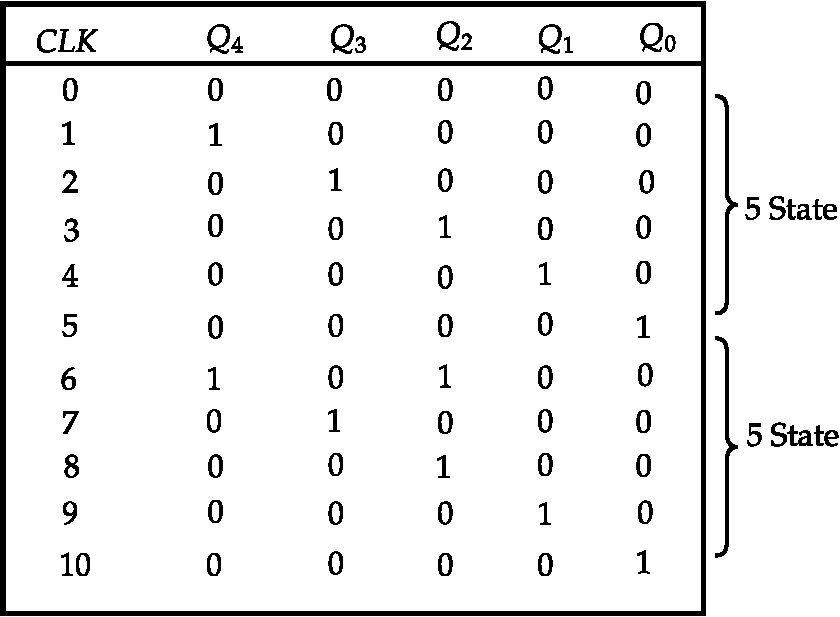
\includegraphics[height=5.7cm,width=8cm]{EDE-39}
\end{figure}
\textbf{Johnson Counter } or (Twisted Ring Counter) or Switch Tail Counter or Creeping Counter or Mobies Counter or Walking Counter.
\begin{figure}[H]
	\centering
	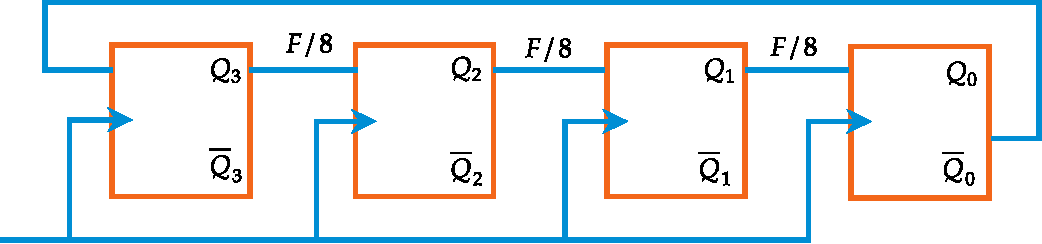
\includegraphics[height=2.4cm,width=9.5cm]{EDE-35}
\end{figure}
\subsubsection{ Equivalent Circuit: }
\begin{figure}[H]
	\centering
	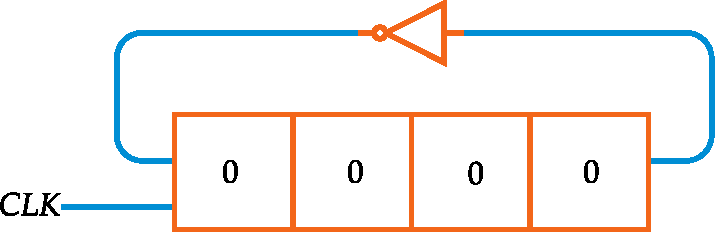
\includegraphics[height=2.4cm,width=7cm]{EDE-36}
\end{figure}
\subsubsection{ Truth Table : }
\begin{figure}[H]
	\centering
	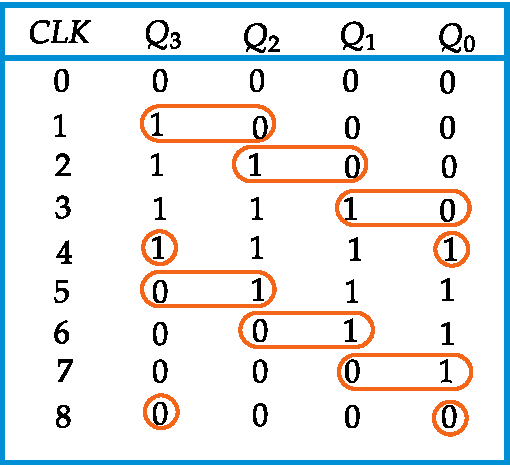
\includegraphics[height=5cm,width=5cm]{EDE-37}
\end{figure}
In Johnson counter with $n$-flip-flop maximum possible states are $2 n$ states or maximum uses states. Unused states are $2^{n}-2 n$.\\
$50 \%$ duty cycle.\\
When a Johnson counter is working in uses state the operation frequency $f / 2 n$.\\
 \end{enumerate}










\newpage
\begin{abox}
	Practise set-1
\end{abox}
\begin{enumerate}
	\item A signal of frequency $10 k H z$ is being digitalized by an A/D converter. A possible sampling time which can be used is
	{	\exyear{NET/JRF(JUNE-2011)}}
	\begin{tasks}(4)
		\task[\textbf{A.}] $100 \mu s$
		\task[\textbf{B.}] $40 \mu s$
		\task[\textbf{C.}] $60 \mu \mathrm{s}$
		\task[\textbf{D.}] $200 \mu s$
	\end{tasks}
	\item Consider the digital circuit shown below in which the input $C$ is always high (1).\\
	\begin{figure}[H]
		\centering
		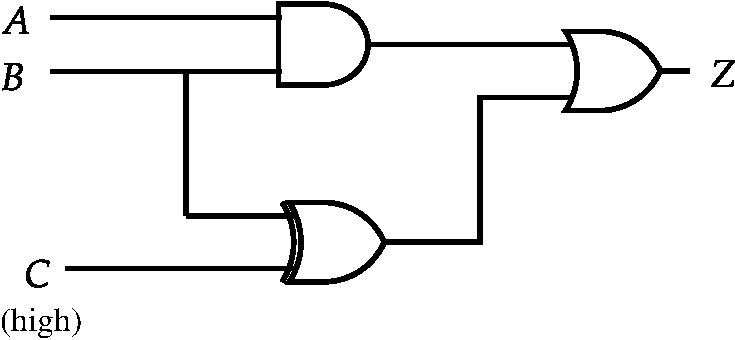
\includegraphics[height=3cm,width=7cm]{diagram-20211018-crop}
	\end{figure}
	The truth table for the circuit can be written as
	\begin{align*}
	\renewcommand*{\arraystretch}{1.2}
	\begin{tabular}{|p{1.5cm}|p{1.5cm}|p{1.5cm}|}
	\hline $\mathrm{A}$ & $\mathrm{B}$ & $\mathrm{Z}$ \\
	\hline 0 & 0 & 1 \\
	\hline 0 & 1 & 0 \\
	\hline 1 & 0 & 1 \\
	\hline 1 & 1 & 1 \\
	\hline
	\end{tabular}
	\end{align*}
	The entries in the $Z$ column (vertically) are
	{	\exyear{NET/JRF(JUNE-2011)}}
	\begin{tasks}(4)
		\task[\textbf{A.}]  1010
		\task[\textbf{B.}] 0100
		\task[\textbf{C.}] 1111
		\task[\textbf{D.}] 1011
	\end{tasks}
	\item A counter consists of four flip-flops connected as shown in the figure:\\
	\begin{figure}[H]
		\centering
		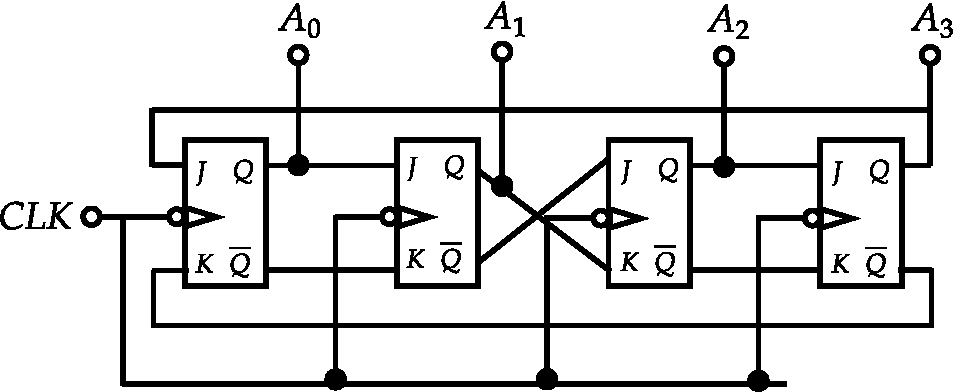
\includegraphics[height=3.5cm,width=7.5cm]{diagram-20211018(3)-crop}
	\end{figure}
	If the counter is initialized as $A_{0} A_{1} A_{2} A_{3}=0110$, the state after the next clock pulse is
	{\exyear{NET/JRF(DEC-2011)}}
	\begin{tasks}(4)
		\task[\textbf{A.}] 1000
		\task[\textbf{B.}]  0001
		\task[\textbf{C.}] 0011
		\task[\textbf{D.}] 1100
	\end{tasks}
	\item The output, $\mathrm{O}$, of the given circuit in cases I and II, where\\
	\textbf{Case I:}\quad $\mathrm{A}, \mathrm{B}=1 ; \mathrm{C}, \mathrm{D}=0 ; \mathrm{E}, \mathrm{F}=1$ and $\mathrm{G}=0$\\
	\textbf{Case II:}\quad $\mathrm{A}, \mathrm{B}=0 ; \mathrm{C}, \mathrm{D}=0: \mathrm{E}, \mathrm{F}=0$ and $\mathrm{G}=1$ are respectively.
	{\exyear{NET/JRF(JUNE-2012)}}
		\begin{tasks}(4)
			\task[\textbf{A.}] 1,0
			\task[\textbf{B.}] 0,1
			\task[\textbf{C.}] 0,0
			\task[\textbf{D.}] 1,1
		\end{tasks}
	\begin{minipage}{0.45\textwidth}
		\begin{figure}[H]
			\centering
			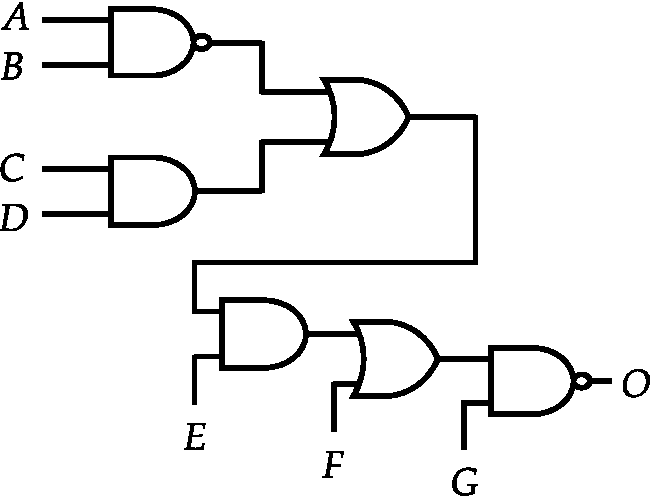
\includegraphics[height=4cm,width=5.5cm]{e-11}
		\end{figure}
	\end{minipage}
	\item  The logic circuit shown in the figure below Implements the Boolean expression
	{\exyear{NET/JRF(DEC-2012)}}
	\begin{figure}[H]
		\centering
		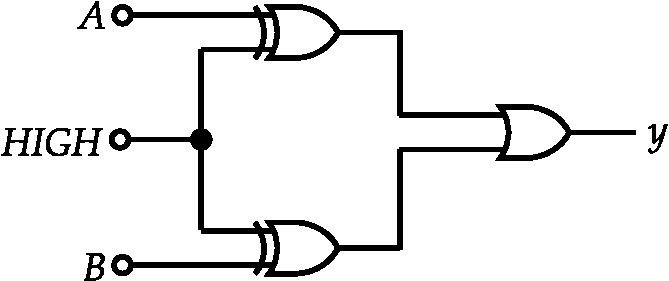
\includegraphics[height=2.5cm,width=6cm]{e-14}
	\end{figure}
	\begin{tasks}(4)
		\task[\textbf{A.}] $y=\overline{A \cdot B}$
		\task[\textbf{B.}] $y=\bar{A} \cdot \bar{B}$
		\task[\textbf{C.}] $y=A \cdot B$
		\task[\textbf{D.}] $y=A+B$
	\end{tasks}
	\item If the analog input to an 8 -bit successive approximation ADC is increased from $1.0 \mathrm{~V}$ to $2.0 \mathrm{~V}$, then the conversion time will
	{\exyear{NET/JRF(JUNE-2013)}}
	\begin{tasks}(2)
		\task[\textbf{A.}] Remain unchanged
		\task[\textbf{B.}] Double
		\task[\textbf{C.}] Decrease to half its original value
		\task[\textbf{D.}] Increase four times
	\end{tasks}
	\item If one of the inputs of a J-K flip flop is high and the other is low, then the outputs $Q$ and $\bar{Q}$
	{	\exyear{NET/JRF(DEC-2013)}}
	\begin{tasks}(1)
		\task[\textbf{A.}] Oscillate between low and high in race around condition
		\task[\textbf{B.}] Toggle and the circuit acts like a $T$ flip flop
		\task[\textbf{C.}] Are opposite to the inputs
		\task[\textbf{D.}] Follow the inputs and the circuit acts like an $R-S$ flip flop
	\end{tasks}
	\item A 4 -variable switching function is given by $f=\sum(5,7,8,10,13,15)+d(0,1,2)$, where $d$ is the do-not-care-condition. The minimized form of $f$ in sum of products (SOP) form is
	{\exyear{NET/JRF(DEC-2013)}}
	\begin{tasks}(4)
		\task[\textbf{A.}] $\bar{A} \bar{C}+\overline{B D}$
		\task[\textbf{B.}] $A \bar{B}+C \bar{D}$
		\task[\textbf{C.}]  $A D+B C$
		\task[\textbf{D.}] $\overline{B D}+B D$
	\end{tasks}
	\item For the logic circuit shown in the below\\
	\begin{figure}[H]
		\centering
		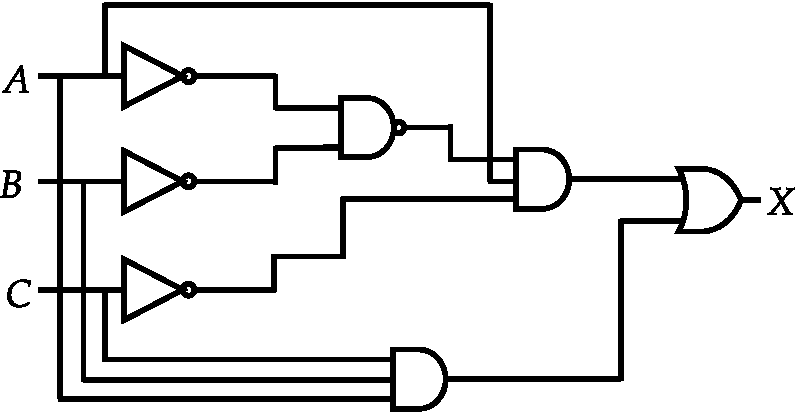
\includegraphics[height=3.5cm,width=7cm]{e-29}
	\end{figure}
	A simplified equivalent circuit is
	{	\exyear{NET/JRF(JUNE-2014)}}
	\begin{tasks}(2)
		\task[\textbf{A.}] 
		\begin{figure}[H]
			\centering
			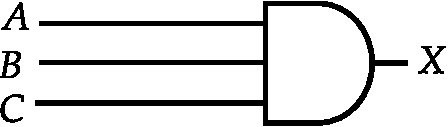
\includegraphics[height=1cm,width=3.3cm]{e-29a}
		\end{figure}
		\task[\textbf{B.}] \begin{figure}[H]
			\centering
			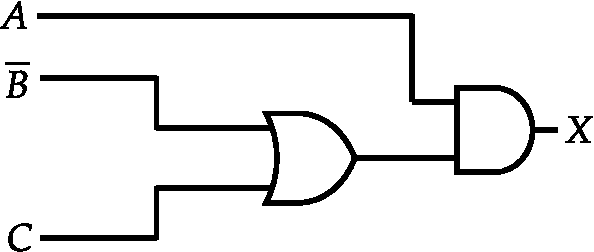
\includegraphics[height=2cm,width=4.5cm]{e-29b}
		\end{figure}
		\task[\textbf{C.}] \begin{figure}[H]
			\centering
			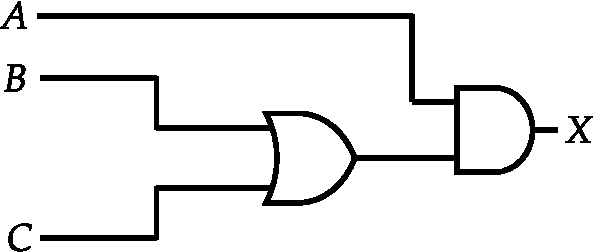
\includegraphics[height=2cm,width=4.5cm]{e-29c}
		\end{figure}
		\task[\textbf{D.}] \begin{figure}[H]
			\centering
			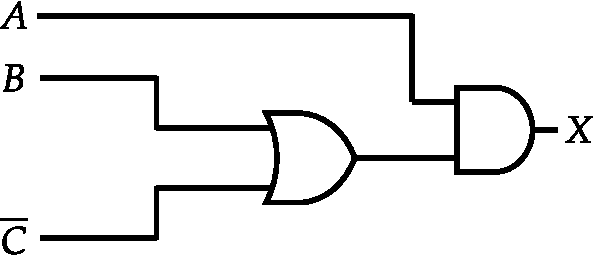
\includegraphics[height=2cm,width=4.5cm]{e-29d}
		\end{figure}
	\end{tasks}
	\item The state diagram corresponding to the following circuit is
	{	\exyear{NET/JRF(DEC-2015)}}
	\begin{figure}[H]
		\centering
		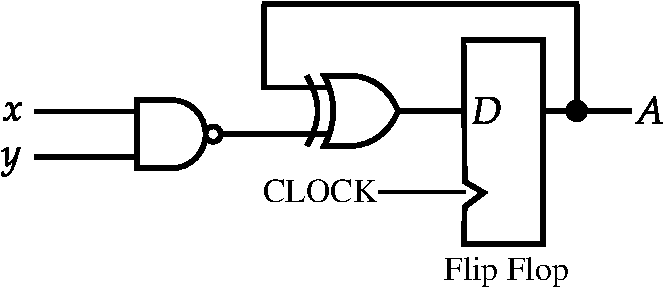
\includegraphics[height=3cm,width=6.5cm]{e41}
	\end{figure}
	\begin{tasks}(2)
		\task[\textbf{A.}] \begin{figure}[H]
			\centering
			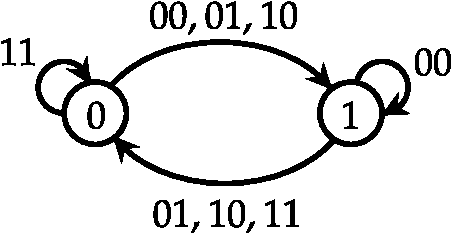
\includegraphics[height=2cm,width=3.8cm]{e41a}
		\end{figure}
		\task[\textbf{B.}] \begin{figure}[H]
			\centering
			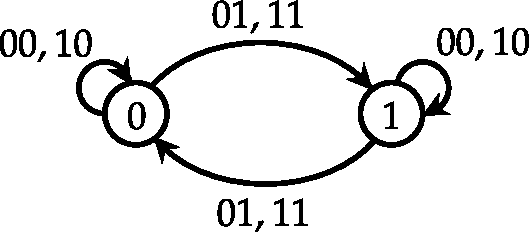
\includegraphics[height=2cm,width=3.8cm]{e41b}
		\end{figure}
		\task[\textbf{C.}] \begin{figure}[H]
			\centering
			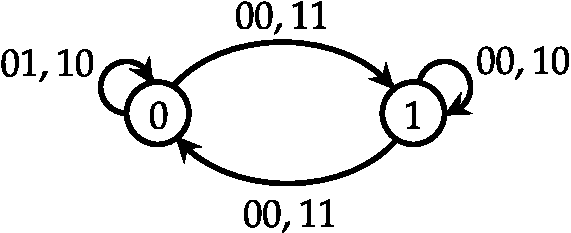
\includegraphics[height=2cm,width=3.8cm]{e41c}
		\end{figure}
		\task[\textbf{D.}] \begin{figure}[H]
			\centering
			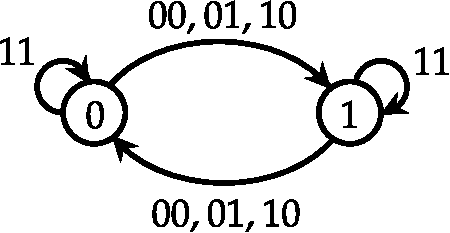
\includegraphics[height=2cm,width=3.8cm]{e41d}
		\end{figure}
	\end{tasks}
	\item In the schematic figure given below, assume that the propagation delay of each logic gate is $t_{\text {gate }}$.\\
	\begin{figure}[H]
		\centering
		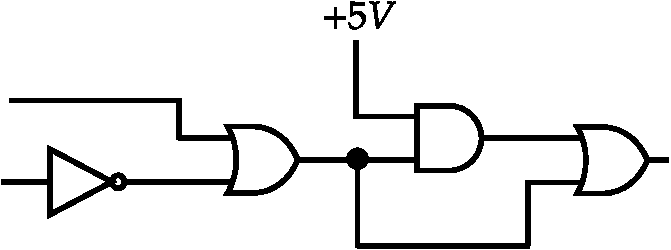
\includegraphics[height=2.5cm,width=5cm]{e44}
	\end{figure}
	The propagation delay of the circuit will be maximum when the logic inputs $A$ and $B$ make the transition
	{\exyear{NET/JRF(JUNE-2016)}}
	\begin{tasks}(2)
		\task[\textbf{A.}] $(0,1) \rightarrow(1,1)$
		\task[\textbf{B.}] $(1,1) \rightarrow(0,1)$
		\task[\textbf{C.}] $(0,0) \rightarrow(1,1)$
		\task[\textbf{D.}] 	$(0,0) \rightarrow(0,1)$
	\end{tasks}
	\item Which of the following circuits implements the Boolean function
	$$F(A, B, C)=\sum(1,2,4,6) ?$$
	{	\exyear{NET/JRF(DEC-2016)}}
	\begin{tasks}(2)
		\task[\textbf{A.}] \begin{figure}[H]
			\centering
			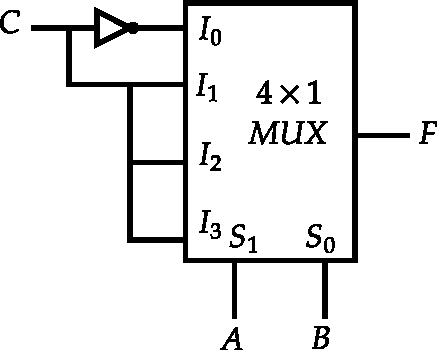
\includegraphics[height=3.3cm,width=4.5cm]{e47a}
		\end{figure}
		\task[\textbf{B.}] \begin{figure}[H]
			\centering
			\includegraphics[height=3.3cm,width=4.5cm]{e47b}
		\end{figure}
		\task[\textbf{C.}] \begin{figure}[H]
			\centering
			\includegraphics[height=3.3cm,width=4.5cm]{e47c}
		\end{figure}
		\task[\textbf{D.}] \begin{figure}[H]
			\centering
			\includegraphics[height=3.3cm,width=4.5cm]{e47d}
		\end{figure}
	\end{tasks}
	\item A $2 \times 4$ decoder with an enable input can function as a
	{	\exyear{NET/JRF(JUNE-2017)}}
	\begin{tasks}(2)
		\task[\textbf{A.}] $4 \times 1$ multiplexer
		\task[\textbf{B.}] $1 \times 4$ demultiplexer
		\task[\textbf{C.}] $4 \times 2$ encoder
		\task[\textbf{D.}] $4 \times 2$ priority encoder
	\end{tasks}
	\item In the figures below, $X$ and $Y$ are one bit inputs. The circuit which corresponds to a one bit comparator is
	{	\exyear{NET/JRF(JUNE-2017)}}
	\begin{tasks}(2)
		\task[\textbf{A.}] \begin{figure}[H]
			\centering
			\includegraphics[height=2.8cm,width=5.5cm]{e58a}
		\end{figure}
		\task[\textbf{B.}] \begin{figure}[H]
			\centering
			\includegraphics[height=2.8cm,width=5.5cm]{e58b}
		\end{figure}
		\task[\textbf{C.}] \begin{figure}[H]
			\centering
			\includegraphics[height=2.8cm,width=5.5cm]{e58c}
		\end{figure}
		\task[\textbf{D.}] \begin{figure}[H]
			\centering
			\includegraphics[height=2.8cm,width=5.5cm]{e58d}
		\end{figure}
	\end{tasks}
	\item The circuit below comprises of $D$-flip flops. The output is taken from $Q_{3}, Q_{2}, Q_{1}$ and $Q_{0}$ as shown in the figure.\\
	\begin{figure}[H]
		\centering
		\includegraphics[height=3.6cm,width=9cm]{e66}
	\end{figure}
	the binary number given by the string $Q_{3}, Q_{2}, Q_{1} Q_{0}$ changes for every clock pulse that is applied to the CLK input. If the output is initialized at 0000 , the the corresponding sequence of decimal numbers that repeats itself, is
	{	\exyear{NET/JRF(DEC-2017)}}
	\begin{tasks}(2)
		\task[\textbf{A.}] $3,2,1,0$
		\task[\textbf{B.}] $1,3,7,14,12,8$
		\task[\textbf{C.}] $1,3,7,15,12,14,0$
		\task[\textbf{D.}] $1,3,7,15,14,12,8,0$
	\end{tasks}
	\item In the following $J K$ flip-flop circuit, $J$ and $K$ inputs are tied together to $+V_{C C} .$ If the input is a clock signal of frequency $f$, the frequency of the output $Q$ is
	{	\exyear{NET/JRF(JUNE-2018)}}
	\begin{figure}[H]
		\centering
		\includegraphics[height=3cm,width=6cm]{e69}
	\end{figure}
	\begin{tasks}(4)
		\task[\textbf{A.}] $f$
		\task[\textbf{B.}] $2 f$
		\task[\textbf{C.}] $4 f$,
		\task[\textbf{D.}] $\frac{f}{2}$
	\end{tasks}
	\item Which of the following gates can be used as a parity checker?
	{	\exyear{NET/JRF(JUNE-2018)}}
	\begin{tasks}(2)
		\task[\textbf{A.}] An OR gate
		\task[\textbf{B.}] A NOR gate
		\task[\textbf{C.}] An exclusive OR (XOR) gate
		\task[\textbf{D.}] An AND gate
	\end{tasks}
	\item The full scale of a 3 -bit digital-to-analog (DAC) converter is $7 V$. Which of the following tables represents the output voltage of this 3 -bit DAC for the given set of input bits?
	{	\exyear{NET/JRF(JUNE-2018)}}
	\begin{tasks}(2)
		\task[\textbf{A.}] 
		\begin{align*}
		\begin{tabular}{|p{2cm} |p{2.5cm}|}
		\hline
		Input bits& Output voltage\\\hline
		000&0\\	\hline
		001&1\\	\hline
		010&2\\	\hline
		011&3\\	\hline
		\end{tabular}
		\end{align*}
		\task[\textbf{B.}] 	\begin{align*}
		\begin{tabular}{|p{2cm} |p{2.5cm}|}
		\hline
		Input bits& Output voltage\\\hline
		000&0\\	\hline
		001&1.25\\	\hline
		010&2.5\\	\hline
		011&3.75\\	\hline
		\end{tabular}
		\end{align*}
		\task[\textbf{C.}] 	\begin{align*}
		\begin{tabular}{|p{2cm} |p{2.5cm}|}
		\hline
		Input bits& Output voltage\\\hline
		000&1.25\\	\hline
		001&2.5\\	\hline
		010&3.75\\	\hline
		011&5\\	\hline
		\end{tabular}
		\end{align*}
		\task[\textbf{D.}] 	\begin{align*}
		\begin{tabular}{|p{2cm} |p{2.5cm}|}
		\hline
		Input bits& Output voltage\\\hline
		000&1\\	\hline
		001&2\\	\hline
		010&3\\	\hline
		011&4\\	\hline
		\end{tabular}
		\end{align*}
	\end{tasks}
	\item Consider the following circuit, consisting of an RS flip-flop and two AND gates.\\
	\begin{figure}[H]
		\centering
		\includegraphics[height=2cm,width=7cm]{e74}
	\end{figure}
	Which of the following connections will allow the entire circuit to act as a $JK$  flip-flop?
	{\exyear{NET/JRF(DEC-2018)}}
	\begin{tasks}(1)
		\task[\textbf{A.}]  Connect $Q$ to pin 1 and $\bar{Q}$ to pin 2
		\task[\textbf{B.}] Connect $Q$ to pin 2 and $\bar{Q}$ to pin 1
		\task[\textbf{C.}] Connect $Q$ to $K$ input and $\bar{Q}$ to $J$ input
		\task[\textbf{D.}] Connect $Q$ to $J$ input and $\bar{Q}$ to $K$ input
	\end{tasks}
	\item The truth table below gives the value $Y ( A , B , C)$  where $A , B$ and $C$ are binary variables.
	The output Y can be represented by
	{\exyear{NET/JRF(DEC-2018)}}
	\begin{tasks}(1)
		\task[\textbf{A.}] $Y=\overline{A B} C+\bar{A} B \bar{C}+A \bar{B} C+A B \bar{C}$
		\task[\textbf{B.}] $Y=\bar{A} \bar{B} \bar{C}+\bar{A} B C+A \bar{B} \bar{C}+A B C$
		\task[\textbf{C.}] $Y=\overline{A B C}+\bar{A} B C+A \overline{B C}+A B C$
		\task[\textbf{D.}] $Y=\bar{A} \bar{B} \bar{C}+\bar{A} B \bar{C}+A \overline{B C}+A B \bar{C}$
	\end{tasks}
	\begin{align*}
	\renewcommand*{\arraystretch}{1.2}
	\begin{tabular}{|p{1cm}|p{1cm}|p{1cm}|p{1cm}|}
	\hline$A$ & $B$ & $C$ & $Y$ \\
	\hline 0 & 0 & 0 & 1 \\
	\hline 0 & 0 & 1 & 0 \\
	\hline 0 & 1 & 0 & 0 \\
	\hline 0 & 1 & 1 & 1 \\
	\hline 1 & 0 & 0 & 1 \\
	\hline 1 & 1 & 0 & 0 \\
	\hline 1 & 1 & 1 & 1 \\
	\hline
	\end{tabular}
	\end{align*}
	\item Let Y denote the output in the following logical Circuit.\\
	\begin{figure}[H]
		\centering	\includegraphics[height=3.5cm,width=5cm]{diagram-20211029(5)-crop}
	\end{figure}
	If $Y=A B+\overline{C D}$, the gates $G_{1}$ and $G_{2}$ must, respectively, be
	{\exyear{NET/JRF(JUNE-2019)}}
	\begin{tasks}(2)
		\task[\textbf{A.}] OR and NAND
		\task[\textbf{B.}] NOR and OR
		\task[\textbf{C.}] AND and NAND
		\task[\textbf{D.}] NAND and OR
	\end{tasks}
	\item In the 3 -bit register shown below, $Q_{1}$ and $Q_{3}$ are the least and the most significant bits of the output, respectively.\\
	\begin{figure}[H]
		\centering
		\includegraphics[height=3.5cm,width=8cm]{diagram-20211029(13)-crop}
	\end{figure}
	If $Q_{1}, Q_{2}$ and $Q_{3}$ are set to zero initially, then the output after the arrival of the second falling clock (CLK) edge is
	{\exyear{NET/JRF(JUNE-2020)}}
	\begin{tasks}(4)
		\task[\textbf{A.}]  001
		\task[\textbf{B.}] 100
		\task[\textbf{C.}]  011
		\task[\textbf{D.}]  110
	\end{tasks}
	\item The Boolean equation $Y=\bar{A} B C+\bar{A} B \bar{C}+A \bar{B} \bar{C}+A \bar{B} C$ is to be implemented using only twoinput NAND gates. The minimum number of gates required is
	{\exyear{NET/JRF(JUNE-2020)}}
	\begin{tasks}(4)
		\task[\textbf{A.}] 3
		\task[\textbf{B.}] 4
		\task[\textbf{C.}] 5
		\task[\textbf{D.}] 6
	\end{tasks}
\end{enumerate}
 \colorlet{ocre1}{ocre!70!}
\colorlet{ocrel}{ocre!30!}
\setlength\arrayrulewidth{1pt}
\begin{table}[H]
	\centering
	\arrayrulecolor{ocre}
	\begin{tabular}{|p{1.5cm}|p{1.5cm}||p{1.5cm}|p{1.5cm}|}
		\hline
		\multicolumn{4}{|c|}{\textbf{Answer key}}\\\hline\hline
		\rowcolor{ocrel}Q.No.&Answer&Q.No.&Answer\\\hline
		1&\textbf{B} &2&\textbf{D}\\\hline 
		3&\textbf{B} &4&\textbf{D} \\\hline
		5&\textbf{A} &6&\textbf{A} \\\hline
		7&\textbf{D}&8&\textbf{D}\\\hline
		9&\textbf{D}&10&\textbf{D}\\\hline
		11&\textbf{D} &12&\textbf{B}\\\hline
		13&\textbf{B}&14&\textbf{C}\\\hline
		15&\textbf{D}&16&\textbf{D} \\\hline
		17&\textbf{C}&18&\textbf{A}\\\hline
		19&\textbf{B}&20&\textbf{B}\\\hline
		21&\textbf{B} &22&\textbf{C}\\\hline
		23&\textbf{B}&&\textbf{}\\\hline
	\end{tabular}
\end{table}
\newpage
\begin{abox}
	Practise set-2
\end{abox}
\begin{enumerate}
	\item The voltage resolution of a 12 -bit digital to analog converter (DAC), whose output varies from $-10 V$ to $+10 V$ is, approximately
	{	\exyear{GATE 2010}}
	\begin{tasks}(4)
		\task[\textbf{A.}] $1\  \mathrm{mV}$
		\task[\textbf{B.}] $5 \ \mathrm{mV}$
		\task[\textbf{C.}] $20 \ \mathrm{mV}$
		\task[\textbf{D.}] $100 \ \mathrm{mV}$
	\end{tasks}
	\item For any set of inputs, A and B, the following circuits give the same output, Q, except one. Which one is it?
	{	\exyear{GATE 2010}}
	\begin{tasks}(2)
		\task[\textbf{A.}] \begin{figure}[H]
			\centering
			\includegraphics[height=2.5cm,width=7cm]{diagram-20210912(13)-crop}
		\end{figure}
		\task[\textbf{B.}]\begin{figure}[H]
			\centering
			\includegraphics[height=1.5cm,width=6cm]{diagram-20210912(14)-crop}
		\end{figure}
		\task[\textbf{C.}] \begin{figure}[H]
			\centering
			\includegraphics[height=2.5cm,width=7.5cm]{diagram-20210912(15)-crop}
		\end{figure}
		\task[\textbf{D.}]\begin{figure}[H]
			\centering
			\includegraphics[height=1.5cm,width=6cm]{diagram-20210912(16)-crop}
		\end{figure}
	\end{tasks}
	\item The following Boolean expression
	$$
	Y=A \cdot \bar{B} \cdot \bar{C} \cdot \bar{D}+\bar{A} \cdot B \cdot \bar{C} \cdot D+\bar{A} \cdot \bar{B} \cdot \bar{C} \cdot D+\bar{A} \cdot \bar{B} \cdot C \cdot D+\bar{A} \cdot B \cdot C \cdot D+A \cdot \bar{B} \cdot \bar{C} \cdot D \quad \text { can }
	$$
	be simplified to
	{	\exyear{GATE 2011}}
	\begin{tasks}(2)
		\task[\textbf{A.}] $\bar{A} \bullet \bar{B} \bullet C+A \bullet \bar{D}$
		\task[\textbf{B.}]  $\bar{A} \bullet B \bullet \bar{C}+A \bullet \bar{D}$
		\task[\textbf{C.}] $A \bullet \bar{B} \bullet \bar{C}+\bar{A} \bullet D$
		\task[\textbf{D.}]  $A \bullet \bar{B} \bullet C+\bar{A} \bullet D$
	\end{tasks}
	\item Which one of the following DOES NOT represent an exclusive OR operation for inputs $A$ and $B ?$
	{	\exyear{GATE 2015}}
	\begin{tasks}(4)
		\task[\textbf{A.}] $(A+B) \overline{A B}$
		\task[\textbf{B.}]  $A \bar{B}+B \bar{A}$
		\task[\textbf{C.}] $(A+B)(\bar{A}+\bar{B})$
		\task[\textbf{D.}] $(A+B) A B$
	\end{tasks}
	\item For the digital circuit given below, the output $X$ is
	{	\exyear{GATE 2016}}
	\begin{figure}[H]
		\centering
		\includegraphics[height=3cm,width=7cm]{diagram-20210914(4)-crop}
	\end{figure}
	\begin{tasks}(4)
		\task[\textbf{A.}] $\overline{\bar{A}+B \cdot C}$
		\task[\textbf{B.}] $\overline{\bar{A} \cdot(B+C)}$
		\task[\textbf{C.}] $\overline{A \cdot}(B+C)$
		\task[\textbf{D.}] $A+\overline{(B . C)}$
	\end{tasks}
	\item The minimum number of NAND gates required to construct an OR gate is:
	{	\exyear{GATE 2017}}
	\begin{tasks}(4)
		\task[\textbf{A.}] 2
		\task[\textbf{B.}] 4
		\task[\textbf{C.}] 5
		\task[\textbf{D.}] 3
	\end{tasks}
	\item The logic expression $\bar{A} B C+\bar{A} \bar{B} C+A B \bar{C}+A \bar{B} \bar{C}$ can be simplified to
	{	\exyear{GATE 2018}}
	\begin{tasks}(4)
		\task[\textbf{A.}] $A\  \mathrm{XOR} \ C$
		\task[\textbf{B.}] $A \ \mathrm{AND} \ C$
		\task[\textbf{C.}] 0
		\task[\textbf{D.}] 1
	\end{tasks}
	\item In a 2-to-1 multiplexer as shown below, the output $X=A_{0}$ if $C=0$ and $X=A_{1}$ if $C=1$.\\
	\begin{figure}[H]
		\centering
		\includegraphics[height=3.5cm,width=4cm]{diagram-20210914(13)-crop}
	\end{figure}
	Which one of the following is the correct implementation of this multiplexer?
	{	\exyear{GATE 2018}}
	\begin{tasks}(2)
		\task[\textbf{A.}] \begin{figure}[H]
			\centering
			\includegraphics[height=2cm,width=5.5cm]{diagram-20210914(14)-crop}
		\end{figure}
		\task[\textbf{B.}] \begin{figure}[H]
			\centering
			\includegraphics[height=2cm,width=5.5cm]{diagram-20210914(15)-crop}
		\end{figure}
		\task[\textbf{C.}]\begin{figure}[H]
			\centering
			\includegraphics[height=2cm,width=5.5cm]{diagram-20210914(16)-crop}
		\end{figure}
		\task[\textbf{D.}] \begin{figure}[H]
			\centering
			\includegraphics[height=2cm,width=5.5cm]{diagram-20210914(17)-crop}
		\end{figure}
	\end{tasks}
	\item Consider the following Boolean expression:
	$$
	(\bar{A}+\bar{B})[\overline{A(B+C)}]+A(\bar{B}+\bar{C})
	$$
	It can be represented by a single three-input logic gate. Identify the gate
	{\exyear{GATE 2019}}
	\begin{tasks}(4)
		\task[\textbf{A.}]  AND
		\task[\textbf{B.}] OR
		\task[\textbf{C.}] XOR
		\task[\textbf{D.}] NAND
	\end{tasks}
	\item A 3 - bit analog-to-digital converter is designed to digitize analog signals ranging from $0 V$ to $10 V$. For this converter, the binary output corresponding to an input of $6 V$ is
	{	\exyear{GATE 2019}}
	\begin{tasks}(4)
		\task[\textbf{A.}] 011
		\task[\textbf{B.}] 101
		\task[\textbf{C.}] 100
		\task[\textbf{D.}] 010
	\end{tasks}
	\item 	For the following circuit, the correct logic values for the entries $X_{2}$ and $Y_{2}$ in the truth table areFor the following circuit, the correct logic values for the entries $X_{2}$ and $Y_{2}$ in the truth table are
	{\exyear{GATE 2019}}\\
	\begin{minipage}{0.45\textwidth}
		\begin{figure}[H]
			\centering
			\includegraphics[height=4cm,width=7cm]{diagram-20210914(22)-crop}
		\end{figure}
	\end{minipage}
	\begin{minipage}{0.45\textwidth}
		\begin{figure}[H]
			\centering
			\includegraphics[height=2.5cm,width=6cm]{diagram-20210914(23)-crop}
		\end{figure}
	\end{minipage}
	\begin{tasks}(4)
		\task[\textbf{A.}] 1 and 0
		\task[\textbf{B.}]  0 and 0 
		\task[\textbf{C.}] 0 and 1
		\task[\textbf{D.}] 1 and 1
	\end{tasks}
	\item The net charge of an $n$ -type semiconductor is
{	\exyear{JEST 2012}}
	\begin{tasks}(4)
		\task[\textbf{A.}] Positive
		\task[\textbf{B.}] Zero
		\task[\textbf{C.}] Negative
		\task[\textbf{D.}] Dependent
	\end{tasks}
	\item For the logic circuit shown in figure, the required input condition $(A, B, C)$ to make the output $(X)=1$ is,
{	\exyear{JEST 2015}}
	\begin{figure}[H]
		\centering
		\includegraphics[height=4cm,width=8cm]{diagram-20210816(11)-crop.pdf}
	\end{figure}
	\begin{tasks}(4)
		\task[\textbf{A.}] $1,0,1$
		\task[\textbf{B.}] $0,0,1$
		\task[\textbf{C.}] $1,1,1$
		\task[\textbf{D.}] $0,1,1$
	\end{tasks}
	\item What is $Y$ for the circuit shown below?
	{\exyear{JEST 2017}}
	\begin{figure}[H]
		\centering
		\includegraphics[height=2.5cm,width=7cm]{diagram-20210816(16)-crop}
	\end{figure}
	\begin{tasks}(2)
		\task[\textbf{A.}] $Y=\overline{(A+\bar{B})(\bar{B}+C)}$
		\task[\textbf{B.}]  $Y=\overline{(A+\bar{B})(B+C)}$
		\task[\textbf{C.}] $Y=\overline{(\bar{A}+B)(\bar{B}+C)}$
		\task[\textbf{D.}] $Y=\overline{(A+B)(\bar{B}+C)}$
	\end{tasks}
\end{enumerate}
 \colorlet{ocre1}{ocre!70!}
\colorlet{ocrel}{ocre!30!}
\setlength\arrayrulewidth{1pt}
\begin{table}[H]
	\centering
	\arrayrulecolor{ocre}
	\begin{tabular}{|p{1.5cm}|p{1.5cm}||p{1.5cm}|p{1.5cm}|}
		\hline
		\multicolumn{4}{|c|}{\textbf{Answer key}}\\\hline\hline
		\rowcolor{ocrel}Q.No.&Answer&Q.No.&Answer\\\hline
		1&\textbf{B} &2&\textbf{D}\\\hline 
		3&\textbf{C} &4&\textbf{D} \\\hline
		5&\textbf{B} &6&\textbf{D} \\\hline
		7&\textbf{A}&8&\textbf{A}\\\hline
		9&\textbf{D}&10&\textbf{C}\\\hline
		11&\textbf{A} &12&\textbf{B}\\\hline
		13&\textbf{D}&14&\textbf{A}\\\hline
		
	\end{tabular}
\end{table}
\newpage
\begin{abox}
	Practise set-3
\end{abox}
\begin{enumerate}
		\item For negative edge draw the time diagram of D Flip-Flop?
	\begin{answer}$\left. \right. $\\
		\begin{figure}[H]
			\centering
			\includegraphics[height=1.7cm,width=4cm]{EDE-08}
		\end{figure}
		For negative edge draw time diagram of D type flip flop.
		\begin{figure}[H]
			\centering
			\includegraphics[height=3.2cm,width=7cm]{EDE-09}
		\end{figure}
		If $\mathrm{D}$ is high then output is high. If $\mathrm{D}$ is low output is low.
	\end{answer}
		\item For the positive clock pulse find the timing diagram of JK flip flop.
	\begin{answer}
		\begin{figure}[H]
			\centering
			\includegraphics[height=1.7cm,width=4cm]{EDE-10}
		\end{figure}
		Time diagram of above flip flop.
		\begin{figure}[H]
			\centering
			\includegraphics[height=3.5cm,width=7cm]{EDE-11}
		\end{figure}
	\end{answer}
		\item Consider a latch circuit shown in figure below, which of the following let of input is invalid for circuit.
	\begin{figure}[H]
		\centering
		\includegraphics[height=2.2cm,width=3.4cm]{EDE-12}
	\end{figure}
	\begin{tasks}(2)
		\task[\textbf{a.}]$\mathrm{R}=0, \mathrm{H}=0$
		\task[\textbf{b.}]$\mathrm{R}=0, \mathrm{H}=1$
		\task[\textbf{c.}]$\mathrm{R}=1, \mathrm{H}=1$
		\task[\textbf{d.}] $\mathrm{R}=1, \mathrm{H}=0$
	\end{tasks}
	\begin{answer}$\left. \right. $\\
		$\begin{array}{|c|c|c|c|}
		\hline R & H & Q & Q \text{ or } Q^{n+1} \\
		\hline 0 & 0 & 0 & 0 \\
		\hline 0 & 0 & 1 & 0 \\
		\hline 0 & 1 & 0 & 0 \\
		\hline 0 & 1 & 1 & 1 \\
		\hline 1 & 0 & 0 & X \\
		\hline 1 & 0 & 1 & X \\
		\hline 1 & 1 & 0 & 1 \\
		\hline 1 & 1 & 1 & 1 \\
		\hline
		\end{array}$\\
		\end{answer}
		\item Design MOD-6 UP Counter:
	\begin{answer}	$\left. \right. $\\
		\begin{figure}[H]
			\centering
			\includegraphics[height=2.7cm,width=11cm]{EDE-19}
		\end{figure}
	\end{answer}
		\item Find MOD of the counter:
	\begin{figure}[H]
		\centering
		\includegraphics[height=2.5cm,width=7cm]{EDE-23}
	\end{figure}
	\begin{tasks}(4)
		\task[\textbf{a.}]1
		\task[\textbf{b.}]2
		\task[\textbf{c.}]3
		\task[\textbf{d.}] 4
	\end{tasks}
	\begin{answer}
		\begin{align*}
		\text { Module of counter } \rightarrow 3, J_{0}&=\bar{Q}_{1}, \bar{J}_{1}=Q_{0}, K_{0}=1, K_{1}=1\\
		\text{	Let initially counter is at}&
		\begin{array}{cc}Q_{1} & Q_{0} \\ 0 & 0\end{array}\\
		\text{i.e. }J_{0}=1
		\qquad\mathrm{J}_{1}=0\\
		\mathrm{K}_{0}=1
		\qquad\mathrm{K}_{1}=1\\
		\text{After one clock pulse}\\
		Q_{0}=1, Q_{1}=0, J_{0}&=1, J_{1}=1, K_{0}=1, K_{1}=1\\
		\text{After two clock pulse}\\
		Q_{0}=0, Q_{1}=1, J_{0}&=0, J_{1}=0, K_{0}=1, K_{1}=1, Q_{0}=0, Q_{1}=1\\
		\text{So reading}\begin{array}{|ll|ll|}
		\hline 0 & 0 & 0 & 0 \\
		1 & 0 & 0 & 1 \\
		0 & 1 & 1 & 0 \\
		0 & 0 & 0 & 0 \\
		\hline
		\end{array}\text{ MOD-3 Counter}
		\end{align*}
	\end{answer}
		\item The circuit shown in figure below is
	\begin{figure}[H]
		\centering
		\includegraphics[height=2.4cm,width=6.5cm]{EDE-38}
	\end{figure}
	\begin{tasks}(2)
		\task[\textbf{a.}]a MOD-2 counter
		\task[\textbf{b.}]A MOD- 3 counter
		\task[\textbf{c.}] Generate sequence $00,10,01,01 \ldots$
		\task[\textbf{d.}] Generate sequence $00,10,00,00 \ldots$.
	\end{tasks}
	\begin{answer}
		The truth table is shown below:\\\\
		\begin{tabular}{p{3cm}p{3cm}p{3cm}}
			Present State&Flip Flop Input&Next State\\
			$Q_A\quad Q_B$&	$T_A\quad T_B$&	$Q_A^+\quad Q_B^+$\\
			0\quad 0&0\quad 1&0\quad 1\\
			0\quad 1&1\quad 1&1\quad 0\\
			1\quad 0&1\quad 0&0\quad 0\\
			1\quad 1&1\quad 1&0\quad 0
		\end{tabular}
	\end{answer}
	 \item Consider a sequential circuit shown in figure. Initially all the flip-flop are reset output $Q_{0} Q_{1} Q_{2}$ after $5^{\text {th }}$ clock pulse is
	\begin{figure}[H]
		\centering
		\includegraphics[height=2.7cm,width=8.5cm]{EDE-24}
	\end{figure}
	\begin{tasks}(4)
		\task[\textbf{a.}]100
		\task[\textbf{b.}]101
		\task[\textbf{c.}]110
		\task[\textbf{d.}] 111
	\end{tasks}
	\begin{answer}
		This is a 3 bit counter, so the output sequence is\\
		$\begin{array}{|llll|}
		\hline \text { CLK } & \mathrm{Q}_{2} & \mathrm{Q}_{1} & \mathrm{Q}_{0} \\
		\hline \text { Initially } & 0 & 0 & 0 \\
		1 & 0 & 0 & 1 \\
		2 & 0 & 1 & 0 \\
		3 & 0 & 1 & 1 \\
		4 & 1 & 0 & 0 \\
		5 & 1 & 0 & 1 \\
		6 & 1 & 1 & 0 \\
		7 & 1 & 1 & 1 \\
		\hline
		\end{array}$
	\end{answer}
	\item The counter shown in figure below is a
	\begin{figure}[H]
		\centering
		\includegraphics[height=2.7cm,width=8cm]{EDE-26}
	\end{figure}
	\begin{tasks}(2)
		\task[\textbf{a.}] MOD-8 up counter
		\task[\textbf{b.}]MOD-8 down counter
		\task[\textbf{c.}]MOD-6 up counter
		\task[\textbf{d.}] MOD-6 down counter
	\end{tasks}
	\begin{answer}$\left. \right. $\\
		$\begin{array}{|c|c|c|c|}
		\hline F F C & F F B & F F A & \\
		\hline J K \bar{C} & J K \bar{B} & J K \bar{A} & C^{+} B^{+} A^{+} \\
		\hline 111 & 111 & 111 & 111 \\
		000 & 000 & 110 & 110 \\
		000 & 110 & 111 & 101 \\
		000 & 001 & 110 & 100 \\
		111 & 111 & 111 & 011 \\
		001 & 000 & 110 & 010 \\
		001 & 110 & 111 & 001 \\
		000 & 001 & 110 & 000 \\
		\hline
		\end{array}$
	\end{answer}
	\item The frequency of the pulse at $\mathrm{Z}$ in the N/W. Show in figure below is
	\begin{figure}[H]
		\centering
		\includegraphics[height=1.1cm,width=13.5cm]{EDE-32}
	\end{figure}
	\begin{tasks}(4)
		\task[\textbf{a.}]$10 \mathrm{~Hz}$
		\task[\textbf{b.}]$160 \mathrm{~Hz}$
		\task[\textbf{c.}]$40 \mathrm{~Hz}$
		\task[\textbf{d.}] $5 \mathrm{~Hz}$
	\end{tasks}
	\begin{answer}
		10-bit ring counter is a MOD-10, so it divides the $160 \mathrm{KHz}$ input by 10 . Therefore, $\mathbf{w}=16 \mathrm{KHz}$. The four bit parallel counter is a MOD-16. Thus, the frequency at $x=1 \mathrm{KHz}$, the $\mathrm{MOD}-25$ ripple counter produces a frequency at $y=40 \mathrm{~Hz} .(1 \mathrm{Khz} / 25=40 \mathrm{~Hz})$. The four bit Johnson counter is a MOD-8. This the frequency at $\mathrm{z}=5 \mathrm{~Hz}$.
	\end{answer}
	\item Consider a sequential circuit using three J-K flip-flop and one AND gate shown in figure output of the circuit becomes ' 1 ' after every $N$-clock cycle. The value of $N$ is
	\begin{figure}[H]
		\centering
		\includegraphics[height=2.7cm,width=10cm]{EDE-33}
	\end{figure}
	\begin{tasks}(4)
		\task[\textbf{a.}]4
		\task[\textbf{b.}]7
		\task[\textbf{c.}]8
		\task[\textbf{d.}] 6
	\end{tasks}
	\begin{answer}
		Let initially output is 1 , then\\
		\begin{tabular}{|cllll|}
			\hline CLK & $\mathrm{Q}$ & $\mathrm{Q}_{1}$ & $\mathrm{Q}_{0}$ & $\mathrm{Z}$ \\
			\hline Initially & 0 & 0 & 0 & 1 \\
			\hline 1 & 1 & 1 & 0 & 0 \\
			2 & 0 & 0 & 1 & 0 \\
			3 & 1 & 0 & 0 & 0 \\
			4 & 0 & 1 & 0 & 0 \\
			5 & 1 & 0 & 1 & 0 \\
			6 & 0 & 0 & 0 & \\
			\hline
		\end{tabular}
	\end{answer}
	

	
\end{enumerate}